\documentclass[times, utf8, zavrsni, english]{fer}
\usepackage{booktabs}
\usepackage{graphicx}
\graphicspath{ {./images/} }

\begin{document}

% TODO: Navedite broj rada.
\thesisnumber{000}

% TODO: Navedite naslov rada.
\title{Application of NLP to threat classification from cybersecurity records}

% TODO: Navedite svoje ime i prezime.
\author{Mirta Medak}

\maketitle

% Ispis stranice s napomenom o umetanju izvornika rada. Uklonite naredbu \izvornik ako želite izbaciti tu stranicu.
\izvornik

% Dodavanje zahvale ili prazne stranice. Ako ne želite dodati zahvalu, naredbu ostavite radi prazne stranice.
\zahvala{}

\tableofcontents

\chapter{Introduction}
Every entity that is dependent on a computer system, from corporations to individuals, could be a subject to cyberattacks. \\
In 2018 there were 80,000 cyberattacks per day or over 30 million attacks per year. [1] During the CoVid-19 pandemic, cybercrime went up 600 \%, as PurpleSec suggests. [2] \\
As technology evolves, more various threats to its security emerge.
Tracking, describing, and evaluating these threats is of use when developing defense systems and making business decisions. \\

\section{Common Vulnerabilities and Exposures System}
A \textbf{vulnerability} is a weakness in a computer system, that an attacker can exploit to execute malicious commands, access data in an unauthorized way, or perform other types of cyber attacks. [4,5] \\
A \textbf{threat} is any circumstance or event which has the potential to compromise system security. [6] \\
In order to tackle the cybersecurity problems in a more organized manner, a system of \emph{CVE (Common Vulnerability and Exposure)} has been developed. \\
The \emph{MITRE Corporation} maintains a public database of an increasing number of CVE records. \\
A CVE record includes an ID, a brief description of the vulnerability, and references.

\section{Common Vulnerability Scoring System}
In order to manipulate and prioritize vulnerabilities in a system, the metric of the Common Vulnerability Scoring System (CVSS) score is used. This metric estimates how "dangerous" exploitation of a vulnerability is. CVSS is an emerging standard of vulnerability comparison. [8] \\
CVSS is divided in three groups: \emph{Base, Temporal and Environmental score}. 
\textbf{Base Score} group shows the traits of the vulnerability that do not change over time and are not dependent on the environment. [9] Predicting the base score will be the subject of this research. \\

\begin{figure}[h]
	\caption{There are eight CVSS Base submetrics:}
	\centering
	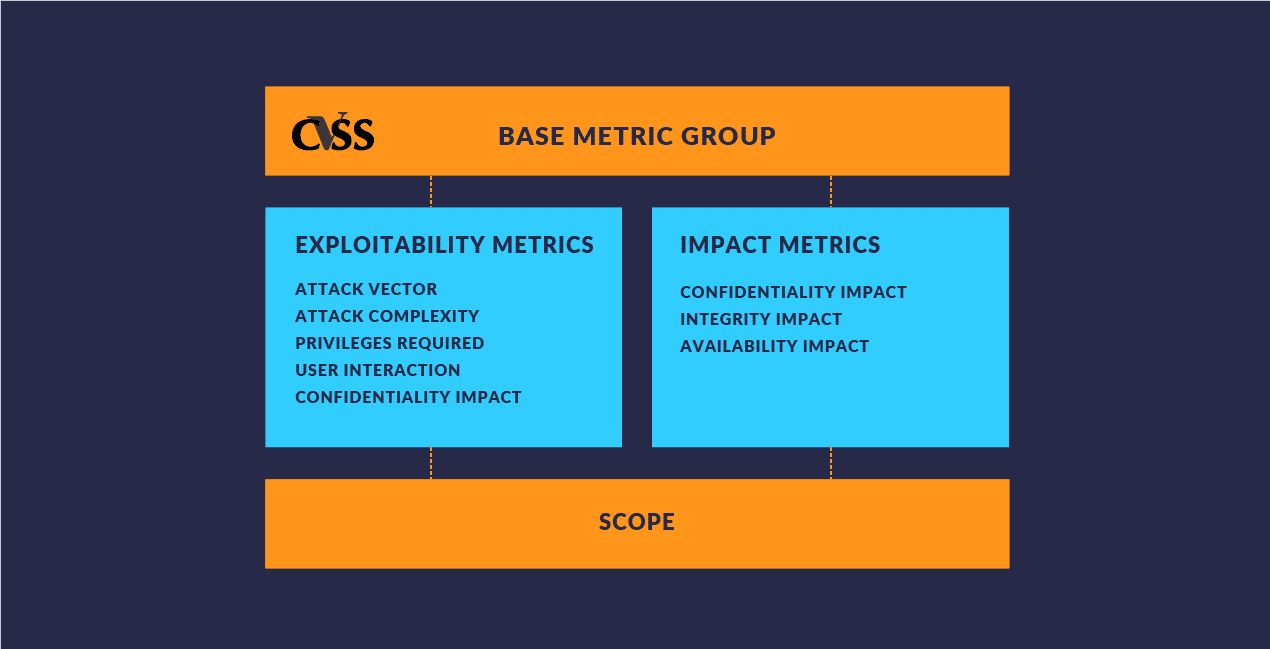
\includegraphics[scale=0.25]{CVSS-Base-Metric-Group}
\end{figure}
Each submetric is assigned by experts. E. g., attack complexity can be assigned as High or Low. The submetrics values all add a different weight to the score. This ratio of how much each submetric matters, is decided by engineers. This formula is then used to compute the score. [Bozorgi et al.] \\
Atefeh Khazaei et al. show an important concern in their work [8]: the CVSS calculation \textbf{can be subjective}.
Moreover, the annotation requires experts and time, which is prolonging the process and is costly. \\
Sometimes, all of the information needed to compute CVSS scores may not be available. Many vulnerabilities aren't assigned the score at all. [7, 10] \\
That is why it would be helpful if CVSS score is automatically decided based on the description of the vulnerability.

In this research, NLP methods are used to predict the CVSS Base score by analyzing the description from the CVE record. \\
BERT classification model has proven to be 90-95 \% accurate in predicting the submetrics using the description of the vulnerability.

\chapter{Related work}
Inspiration to do this research has been given by the study of Cook, Bryan, et al., who have developed an application that takes any vulnerability description and gives its CVSS score. [10] They used BERT classification to predict the Base score submetrics. The CVSS score was then calculated using the hard-coded CVSS formula and the predicted submetrics results. They have achieved accuracy in the 0.90 range. \\

Another study developing an objective method of CVSS score calculation, written by Khazaei et al. [], used Support Vector Machine, Random-Forest, and fuzzy system. Their model's accuracy was around 0.86. \\

This problem was approached in detail by Bozorgi et al. [] Instead of predicting the CVSS score itself, they have developed a new classification system, using various features of the vulnerability. \\

\chapter{Data}
\section{Data acquisition}
Dataset used has been acquired and prepared by Cook et al., when used in their work \emph{Using NLP to Predict the Severity of Cybersecurity Vulnerabilities, 2021.}
Most of the data is publicly available and maintained by the MITRE organization and the National Institute of Standards of Technology. \\
From the cited research, we find out that at the beginning of 2021, only 50 \% of CVE records had a CVSS score assigned. \\
The datasets were created by human experts and therefore didn't require much preparation or preprocessing. 

\section{Dataset structure}

The dataset has 61616 entries.

\begin{table}[h!]
	\centering
	\begin{tabular}{||c c c ||} 
		\hline
		 & Column Title & Values  \\ [0.5ex] 
		\hline\hline
		
		1 & attack\_vector & physical; adj\_network;   \\
		 & &  local; network \\
		2 & attack\_complexity & high; low  \\
		3 & privileges\_required & high; low; none  \\
		4 & user\_interaction & none; required \\ 
		5 & scope & unchanged; changed \\ 
		6 & confidentiality & high; low; none  \\
		7 & integrity & high; low; none  \\
		8 & availability & high; low; none  \\
		
		\hline\hline
		9 & description & natural language description \\
		10 & base\_score & float from 0 - 10 \\
		\hline
	\end{tabular}
\caption{Columns and their values used in experiments}
\label{table:1}
\end{table}

The first eight entries of Table 3.1. correspond to eight submetrics of CVSS base score.
\section{Dataset analysis}
According to CVSS v3.0 Ratings [nistgovstranica] the severity is classified in the following ranges:
\begin{table}[h!]
	\centering
	\begin{tabular}{| c c c ||} 
		\hline
		Severity & Base score range & No. of examples\\ [0.5ex] 
		\hline\hline
		
		None & 0.0 & 0  \\
		Low &  0.1-3.9 & 1115 \\
		Medium & 4.0-6.9 & 24232  \\
		High & 7.0-8.9  & 26793 \\
		Critical & 9.0-10.0 & 9476\\
		\hline
	\end{tabular}
	\caption{CVSS range classification and number of examples in each class}
	\label{table:2}
\end{table}
From Table 2. we can clearly see that the medium to high scores prevail. 
% TODO: Dodati koji graf.

\chapter{Models}

\section{Baseline Models}
\section{Support Vector Regression}
\subsection{word2vec}
\subsection{Support Vector Machines}
\subsection{SVR, LinearSVR, SGDRegressor}

\section{BERT}
\subsection{BERT architecture}
\subsection{BERT for regression}
\subsection{BERT classification}

\chapter{Experiments and results}

\chapter{Conclusion}
Conclusion.

\bibliography{literatura}
\bibliographystyle{plainnat}

\listoffigures
\begin{abstract}
Abstract.

\keywords{Keywords.}
\end{abstract}

% TODO: Navedite naslov na hrvatskom jeziku.
\hrtitle{Naslov}
\begin{sazetak}
Sažetak na hrvatskom jeziku.

\kljucnerijeci{Ključne riječi, odvojene zarezima.}
\end{sazetak}

\end{document}
